%% This is an example first chapter.  You should put chapter/appendix that you
%% write into a separate file, and add a line \include{yourfilename} to
%% main.tex, where `yourfilename.tex' is the name of the chapter/appendix file.
%% You can process specific files by typing their names in at the 
%% \files=
%% prompt when you run the file main.tex through LaTeX.
%   _____ ______      __  _____             
%  / ____|  _ \ \    / / |  __ \            
% | |    | |_) \ \  / /  | |  | | _____   __
% | |    |  _ < \ \/ /   | |  | |/ _ \ \ / /
% | |____| |_) | \  /    | |__| |  __/\ V / 
%  \_____|____/   \/     |_____/ \___| \_/  
%                                           
%                                           

\chapter{Specific Aim 1: Scott Caan}

\section{Scott Caan}

\subsection{Introduction and study design}
 Scott Caan?\cite{caan4}
\subsection{Methods}
\begin {figure}[htbp]
\centering
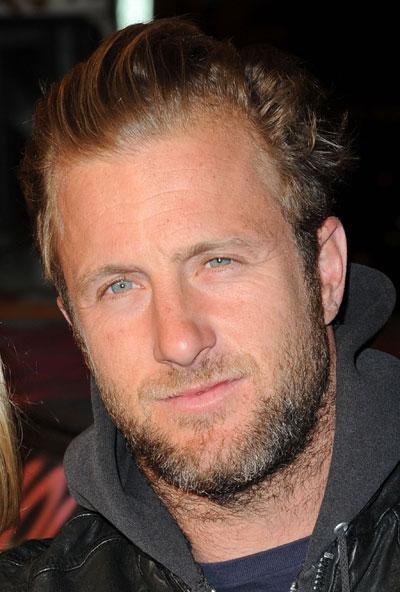
\includegraphics[scale=.5]{scottcaan5}
\caption{Scott Caan}
\label{fig5}
\centering
\end{figure}
Scott Caan...
\subsection{Results and discussion}


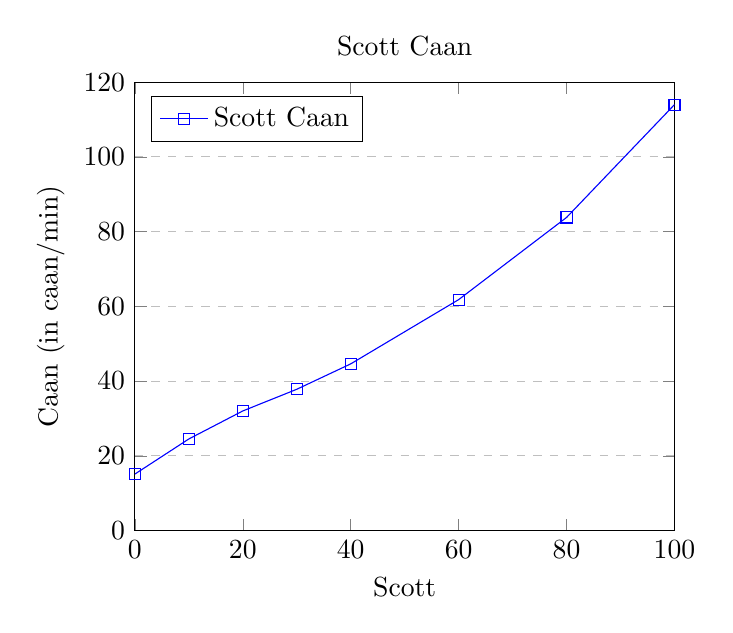
\begin{tikzpicture}
\begin{axis}[
    title={Scott Caan},
    xlabel={Scott},
    ylabel={Caan (in caan/min)},
    xmin=0, xmax=100,
    ymin=0, ymax=120,
    xtick={0,20,40,60,80,100},
    ytick={0,20,40,60,80,100,120},
    legend pos=north west,
    ymajorgrids=true,
    grid style=dashed,
]
 
\addplot[
    color=blue,
    mark=square,
    ]
    coordinates {
    (0,15.1)(10,24.5)(20,32)(30,37.8)(40,44.6)(60,61.8)(80,83.8)(100,114)
    };
    \legend{Scott Caan}
 
\end{axis}
\end{tikzpicture}



Scott Caan.
\subsection{Conclusion}
Scott Caan!\cite{caan5}